% =====================================================================
% Manuscrito para EPIDEMIOLOGIA E SERVIÇOS DE SAÚDE (RESS)
% Tipo: Artigo Original (estudo ecológico)
% Versão independente, reformatada a partir das normas da RESS
% (SciELO/Ministério da Saúde) e revisada segundo parecer de pares e
% comentários de coautoria (DeCS, clareza metodológica, reframe para
% Saúde Coletiva, distinção desigualdade x iniquidade, lei dos
% cuidados inversos, caveat ecológico, padronização de unidades).
%
% Normas RESS aplicadas (artigo original):
%   - até 3.500 palavras (excluindo resumo, tabelas, figuras, refs)
%   - resumo estruturado, parágrafo único, até 250 palavras
%     (Objetivo, Métodos, Resultados, Conclusão)
%   - 5 palavras-chave dos Descritores em Ciências da Saúde (DeCS)
%   - referências estilo Vancouver [colchetes], com DOI; até 30
%   - estrutura IMRaD: Introdução, Métodos, Resultados, Discussão
%   - até 5 tabelas e figuras (combinadas)
%   - CRediT; declaração de ética
%
% >>> Dados de autoria completos: afiliação (pesquisadores
%     independentes), cidade/estado, titulação, cargo e ORCID dos 4
%     autores. Resta apenas confirmar a distribuição de papéis CRediT.
%
% Compilação: tectonic equipamentos-rm-parkinson-RESS.tex
% =====================================================================

\documentclass[12pt,a4paper,oneside]{article}

\usepackage[T1]{fontenc}
\usepackage[utf8]{inputenc}
\usepackage[brazilian]{babel}
\usepackage{newtxtext}
\usepackage{newtxmath}
\usepackage[section]{placeins}
\usepackage[a4paper,top=2.5cm,bottom=2.5cm,left=3cm,right=2.5cm]{geometry}
\usepackage{setspace}
\usepackage{indentfirst}
\usepackage{titlesec}
\usepackage{caption}
\usepackage{booktabs}
\usepackage{array}
\usepackage{graphicx}
\usepackage{xcolor}
\usepackage{fancyhdr}
\usepackage[colorlinks=true,urlcolor=blue!55!black,linkcolor=black,
            citecolor=black,breaklinks=true]{hyperref}
\usepackage{url}
\usepackage{xurl}
\Urlmuskip=0mu plus 1mu\relax

\graphicspath{{figures-equipamentos-rm/}}

\onehalfspacing
\setlength{\parindent}{1.25cm}
\setlength{\parskip}{0pt}

\titleformat{\section}{\normalfont\bfseries\large\uppercase}{\thesection}{0.6em}{}
\titleformat{\subsection}{\normalfont\bfseries\normalsize}{\thesubsection}{0.6em}{}
\titlespacing*{\section}{0pt}{16pt}{8pt}
\titlespacing*{\subsection}{0pt}{10pt}{5pt}

\captionsetup[table]{labelfont=bf,name=Tabela,labelsep=endash,
                     position=above,justification=centering,font=small}
\captionsetup[figure]{labelfont=bf,name=Figura,labelsep=endash,
                      position=below,justification=centering,font=small}
\captionsetup{skip=6pt}

\pagestyle{fancy}\fancyhf{}
\fancyfoot[C]{\small\thepage}
\renewcommand{\headrulewidth}{0pt}

\newcounter{bibctr}
\newcommand{\refitem}[1]{\refstepcounter{bibctr}\noindent%
  \hangindent=0.7cm\hangafter=1\label{#1}\textbf{\thebibctr.}\ }

\begin{document}

% =====================================================================
% PÁGINA DE ROSTO
% =====================================================================
\thispagestyle{fancy}
\begin{singlespace}

\begin{center}
{\small\textsc{Artigo Original}}

\vspace{10pt}
{\large\bfseries Iniquidade regional no acesso à neuroimagem para a
doença de Parkinson no Brasil, 2013\textendash 2025: estudo ecológico
de base nacional\par}

\vspace{8pt}
{\itshape Regional inequity in access to neuroimaging for Parkinson's
disease in Brazil, 2013\textendash 2025: a nationwide ecological
study\par}

\vspace{8pt}
{\footnotesize\textbf{Título resumido:} Neuroimagem e Parkinson no SUS}

\vspace{14pt}
\textbf{Leonardo Chalhoub} \quad\textbullet\quad \textbf{Alexandre Maciel Rolim}\\[4pt]
\textbf{Luis Fernando Kranz} \quad\textbullet\quad \textbf{Jefferson Korte}
\end{center}

\vspace{0.4cm}
\small
\noindent Todos os autores atuam como \textbf{pesquisadores
independentes}, Brasil.\\[4pt]
\noindent\textit{Leonardo Chalhoub} \textemdash{} Pesquisador
independente; \textit{Expert Data Engineer}. Mestre em Administração
(Finanças), Universidade Federal do Rio Grande do Sul (UFRGS);
graduando em Engenharia de Software, Universidade Estácio de Sá
(2023\textendash 2026). Rio de Janeiro, RJ, Brasil.
ORCID: 0000-0003-0484-158X.\\[2pt]
\noindent\textit{Alexandre Maciel Rolim} \textemdash{} Pesquisador
independente; Tecnólogo em Radiologia. Mestre em Proteção Radiológica,
Instituto Federal de Santa Catarina (IFSC). Florianópolis, SC, Brasil.
ORCID: 0009-0000-3983-4713.\\[2pt]
\noindent\textit{Luis Fernando Kranz} \textemdash{} Pesquisador
independente; Tecnólogo em Radiologia. Mestre em Administração,
Universidade Federal do Rio Grande do Sul (UFRGS). Porto Alegre, RS,
Brasil. ORCID: 0009-0009-6015-3141.\\[2pt]
\noindent\textit{Jefferson Korte} \textemdash{} Pesquisador
independente; estudante de Ciência da Computação, Universidade
Tecnológica Federal do Paraná (UTFPR). Curitiba, PR, Brasil.
ORCID: 0009-0006-9466-9830.

\vspace{0.5cm}
\noindent\textbf{Correspondência:} Leonardo Chalhoub.
E-mail: leochalhoub@hotmail.com.

\vspace{0.4cm}
\noindent\textbf{Contribuições dos autores (CRediT).}
\textit{L.\ Chalhoub:} conceituação, curadoria de dados, análise
formal, \textit{software}, visualização, redação (rascunho original e
revisão). \textit{A.\,M.\ Rolim:} metodologia, investigação,
validação, redação (rascunho original e revisão).
\textit{L.\,F.\ Kranz:} conceituação, metodologia, supervisão, redação
(revisão). \textit{J.\ Korte:} \textit{software}, curadoria de dados,
visualização, redação (revisão). Todos aprovaram a versão final e
respondem pela integridade do trabalho. \textit{(Distribuição de
papéis a confirmar pelos autores.)}

\vspace{0.4cm}
\noindent\textbf{Conflitos de interesse:} os autores declaram não
haver conflitos de interesse. \textbf{Financiamento:} o estudo não
recebeu financiamento. \textbf{Disponibilidade de dados:} os dados
primários são públicos (CNES/DATASUS; IBGE); código e conjunto
consolidado disponíveis no repositório aberto do projeto.\footnote{%
\url{https://github.com/leonardochalhoub/mirante-dos-dados-br}}

\vspace{0.4cm}
\noindent\textbf{Aspectos éticos:} estudo ecológico baseado
exclusivamente em dados secundários, públicos, agregados e
anonimizados, sem identificação de indivíduos. Nos termos da Resolução
CNS n.\ 510/2016 (art.\ 1º, parágrafo único), pesquisas que utilizam
informações de acesso público, sem identificação de participantes, são
dispensadas de registro e apreciação pelo Sistema CEP/CONEP; não há,
portanto, número de parecer, data de aprovação, número de CAAE ou
registro de consentimento aplicáveis. \textbf{Uso de inteligência
artificial:} ferramentas de IA foram empregadas apenas como apoio à
edição de linguagem e formatação, sem participação na coleta, no
processamento ou na análise dos dados; os autores revisaram
integralmente o conteúdo.

\end{singlespace}

\newpage

% =====================================================================
% RESUMO + DESCRITORES
% =====================================================================
\section*{Resumo}
\begin{singlespace}\small\noindent
\textbf{Objetivo:} quantificar e caracterizar a distribuição regional
do parque instalado de quatro modalidades de neuroimagem relevantes
para o diagnóstico diferencial da doença de Parkinson (DP) no Brasil e
avaliar a equidade do acesso. \textbf{Métodos:} estudo ecológico de
série temporal (2013\textendash 2025), com microdados do Cadastro
Nacional de Estabelecimentos de Saúde (CNES); densidade por milhão de
habitantes (Mhab) a partir de estimativas do IBGE; comparação com
referenciais da OCDE; índice de Kakwani sobre a densidade de
ressonância magnética (RM) \textit{versus} o Índice de Desenvolvimento
Humano (IDH) estadual; e índice de necessidade (casos estimados de DP
por equipamento). \textbf{Resultados:} a densidade nacional de RM
atingiu 18,3/Mhab em 2025, próxima à mediana da OCDE (19,4), mas com
forte gradiente regional: 17 das 27 unidades federativas situaram-se
abaixo da mediana, e Acre (5,7), Roraima (8,1) e Amazonas (8,6) abaixo
de metade desse referencial. O índice de Kakwani foi $+0{,}183$
(IC95\% 0,12\textendash 0,24), indicando distribuição regressiva
pró-rico; o índice de necessidade variou cerca de oito vezes entre os
extremos. \textbf{Conclusão:} a principal barreira ao diagnóstico
diferencial da DP no Brasil não é o volume agregado de equipamentos,
mas a iniquidade espacial do acesso, que tende a se agravar com o
envelhecimento populacional e demanda políticas de regionalização,
padronização de protocolos e telerradiologia.

\vspace{0.35cm}\noindent\textbf{Palavras-chave:} Doença de Parkinson;
Neuroimagem; Acesso aos Serviços de Saúde; Disparidades em Assistência
à Saúde; Sistema Único de Saúde.
\end{singlespace}

\newpage

% =====================================================================
\section{Introdução}
% =====================================================================

A doença de Parkinson (DP) é a condição neurodegenerativa de
crescimento populacional mais acelerado no mundo. Estima-se que o
número de pessoas com DP tenha passado de 3,15 milhões em 1990 para
11,77 milhões em 2021, podendo alcançar cerca de 25 milhões em
2050\,[\ref{ref:gbd}, \ref{ref:su}] \textemdash{} fenômeno que parte
da literatura descreve como uma ``pandemia de Parkinson''. A pressão
não se restringe a países de alta renda: os Estados Unidos projetam a
duplicação de casos até 2030\,[\ref{ref:marras}] e a Europa registra
prevalência de 160 a 250 por 100 mil habitantes\,[\ref{ref:voncamp}],
mas o maior crescimento relativo concentra-se em países de renda
média, pressionados pelo envelhecimento e por sistemas de saúde em
consolidação \textemdash{} contexto em que o Brasil se insere.

Para o Brasil, o estudo longitudinal ELSI-Brazil estimou prevalência
de 0,84\% (IC95\%: 0,64\textendash 1,09) entre indivíduos com 50 anos
ou mais, projetando crescimento de 535.999 casos em 2024 para
1.250.638 em 2060\,[\ref{ref:elsi}]. Como a prevalência cresce
exponencialmente com a idade, e a população com 60 anos ou mais deverá
quase dobrar até 2050\,[\ref{ref:ibge-proj}], o crescimento projetado
da DP traduz-se em aumento expressivo da demanda por diagnóstico
diferencial com suporte de imagem nas próximas duas décadas.

O diagnóstico de DP é clínico\,[\ref{ref:mds}], mas o diagnóstico
\textbf{diferencial} entre a DP idiopática e os parkinsonismos
atípicos (atrofia multissistêmica, paralisia supranuclear progressiva,
demência com corpos de Lewy e degeneração corticobasal) é desafiador
na apresentação inicial\,[\ref{ref:tolosa}] e, segundo as diretrizes
internacionais, requer suporte de neuroimagem
\textit{escalonada}\,[\ref{ref:efns}, \ref{ref:aan}] \textemdash{} o
uso progressivo de modalidades de crescente complexidade e custo. A
ressonância magnética (RM) é o suporte de primeira linha: exclui
mimetizadores estruturais e, com a imagem ponderada por
susceptibilidade, identifica o sinal da ``cauda de andorinha'' (perda
da hiperintensidade do nigrossomo-1), com sensibilidade de 94,6\% e
especificidade de 94,4\%\,[\ref{ref:swallow}]. A tomografia
computadorizada (CT) é alternativa para exclusão de
mimetizadores\,[\ref{ref:saba}]; a DAT-SPECT, adquirida em câmara
gama, é a modalidade mais específica para distinguir a DP de
mimetizadores não degenerativos, e a neuroimagem dopaminérgica normal
é critério de exclusão absoluta de DP\,[\ref{ref:mds},
\ref{ref:catafau}]; e a PET/CT cumpre papel terciário, restrito a
centros de referência\,[\ref{ref:stoessl}].

A distribuição de recursos diagnósticos de alta complexidade no SUS é
historicamente desigual\,[\ref{ref:lopes}], mas a literatura nacional
raramente articula, de forma reproduzível, a oferta instalada de
neuroimagem relevante para a DP com a sua distribuição regional e a
equidade do acesso. Cabe distinguir \textbf{desigualdade} (diferença
observada na distribuição de recursos) de \textbf{iniquidade}
(diferença injusta e evitável, à luz de princípios de justiça
distributiva)\,[\ref{ref:wagstaff}]: o interesse de saúde pública
recai sobre a segunda. Diante disso, este estudo perguntou,
especificamente: (i) qual a densidade per capita de RM, CT, PET/CT e
câmaras gama no Brasil, por unidade federativa (UF), entre
2013\textendash 2025; (ii) como essa densidade se compara a
referenciais internacionais; e (iii) quão equitativamente esses
recursos se distribuem em relação ao desenvolvimento socioeconômico
(IDH) e à carga estimada de DP. O objetivo foi quantificar o parque
instalado dessas modalidades e caracterizar a iniquidade regional do
acesso por meio de indicadores formais de equidade.

% =====================================================================
\section{Métodos}
% =====================================================================

\subsection{Desenho e fontes de dados}

Estudo ecológico, de série temporal, tendo como unidade de análise a
UF. A fonte primária é o módulo de Equipamentos do Cadastro Nacional
de Estabelecimentos de Saúde (CNES/DATASUS), que disponibiliza
microdados mensais por estabelecimento; cada equipamento é
identificado pelas chaves \texttt{TIPEQUIP} (categoria) e
\texttt{CODEQUIP} (código), conforme o catálogo oficial do
DATASUS\,[\ref{ref:datasus-cat}]. Analisaram-se quatro modalidades:
RM (\texttt{1:12}), CT (\texttt{1:11}), PET/CT (\texttt{1:18}) e câmara
gama (\texttt{1:01}), suporte da DAT-SPECT. A janela 2013\textendash 2025
foi escolhida porque, antes de 2013, o preenchimento do módulo de
equipamentos do CNES é descontínuo e inconsistente entre UF, o que
inviabiliza séries comparáveis; o recorte garante uma série estável.
As estimativas anuais de população residente por UF, usadas na
normalização per capita, provêm do IBGE\,[\ref{ref:ibge-pop}].

\subsection{Arquitetura do \textit{pipeline} de dados e
reprodutibilidade}

O processamento apoia-se em um \textit{pipeline} livre, de código
aberto e reproduzível, organizado segundo a arquitetura
\textit{medallion} \textemdash{} \textit{bronze}, \textit{silver} e
\textit{gold}\,[\ref{ref:lakehouse}] \textemdash{}, precedida de uma
camada \textit{Raw} de aterrissagem dos arquivos-fonte; são, ao todo,
quatro camadas de qualidade progressiva (\textit{Raw}, \textit{bronze},
\textit{silver} e \textit{gold}), com posterior serialização da
\textit{gold} para consumo (\textit{export}). O processamento distribuído é
feito em Apache Spark, por meio da \textit{interface} PySpark; a
persistência usa exclusivamente tabelas Delta Lake (sem \textit{Delta
Live Tables} e sem \textit{views} materializadas), o que provê
transações ACID, evolução de esquema e versionamento com ``viagem no
tempo'' (\textit{time travel}). A execução ocorre na plataforma
\textbf{Databricks Free Edition} (camada gratuita do Databricks), com
governança e armazenamento pelo Unity Catalog (\textit{Volumes}); a
orquestração é declarada como código por meio de \textit{Databricks
Asset Bundles}, em que um \textit{job} em cascata encadeia
\texttt{ingestão $\rightarrow$ bronze $\rightarrow$ silver
$\rightarrow$ gold $\rightarrow$ export}, com dependências explícitas
que garantem a ordem de materialização. Por usar exclusivamente a
\textbf{Databricks Free Edition} e ferramentas de código aberto (Apache
Spark, Delta Lake, PySpark), o \textit{pipeline} é integralmente
reproduzível por terceiros sem custo de licença ou de infraestrutura.

\textbf{Camada bronze (dado bruto).} A \textit{bronze} preserva o
registro fiel da fonte: os arquivos mensais por UF, no formato
proprietário DBC (DBF comprimido), trazem os lançamentos por
estabelecimento de saúde. Em volume, a camada \textit{bronze} acumula,
em modo \textit{append-only}, 316.114.382 registros brutos de
equipamentos do CNES (2005\textendash 2025, 27 UF); o recorte das
quatro modalidades de neuroimagem-DP em 2013\textendash 2025
corresponde a 2.520.636 registros brutos, referentes a 17.846
estabelecimentos de saúde distintos. Como o DBC é binário comprimido e não é
legível diretamente pelo mecanismo de ingestão incremental, adota-se um
procedimento em dois estágios. Primeiro, cada DBC é descomprimido para
DBF \textemdash{} via \texttt{pyreaddbc}, que empacota o decodificador
em linguagem C herdado do projeto PySUS \textemdash{} e lido com
\texttt{dbfread}, sendo materializado em Parquet com \textit{pandas},
em conversão paralelizada por processos. Em seguida, o \textit{Auto
Loader} (\texttt{cloudFiles}) varre a pasta de Parquet e faz
\textit{append} incremental na tabela Delta \textit{bronze}, com
\textit{checkpoint} e \textit{schema location} em \textit{Volumes} do
Unity Catalog; a camada é \textbf{string-only}, sem inferência de tipo,
e o modo incremental detecta de forma econômica os novos arquivos dos
\textit{refreshes} mensais. É na \textit{bronze} que residem os dados
brutos por estabelecimento e mês; todas as contagens e densidades
agregadas reportadas nos Resultados são grandezas \textit{derivadas} a
jusante, na camada \textit{gold}, e não leituras diretas do dado bruto.

\textbf{Camada silver (modelagem).} A \textit{silver} agrega pela
chave composta \texttt{(estado, ano, tipequip, codequip)}. A presença
do \texttt{tipequip} é indispensável: as categorias de equipamento
reaproveitam a mesma faixa numérica de \texttt{codequip}, de modo que
usar \texttt{codequip} isolado fundiria categorias distintas
\textemdash{} origem de um erro em versão anterior, em que
\texttt{codequip=42} capturava eletroencefalógrafo no lugar do
equipamento pretendido. Define-se, então, a chave
\texttt{equipment\_key = "tipequip:codequip"} (por exemplo,
\texttt{1:12} para RM), usada em toda a análise. Os identificadores são
normalizados (\texttt{TIPEQUIP} convertido a \textit{string};
\texttt{CODEQUIP} preenchido a dois dígitos) e a deduplicação toma o
\textit{snapshot} mais recente por arquivo de origem. A divisão
público-privada usa a variável \texttt{IND\_SUS}; quando um mesmo
(estabelecimento, mês) apresenta linhas com \texttt{IND\_SUS} 1 e 0,
toma-se o maior valor entre as contagens SUS e privada por
(estabelecimento, mês), evitando dupla contagem. Um \textbf{vocabulário
controlado} (dicionário canônico de equipamentos) mapeia cada
\texttt{(tipequip, codequip)} ao nome do equipamento, sinalizando
combinações ausentes.

\textbf{Camadas gold e export.} A \textit{gold} junta a \textit{silver}
às estimativas populacionais do IBGE e calcula, por \texttt{(estado,
ano, equipment\_key)}, os indicadores analíticos: número de
estabelecimentos distintos, contagem média anual de unidades
(deduplicada por estabelecimento), densidade por milhão de habitantes e
as respectivas versões SUS e privada. É, portanto, a camada em que
ocorre a agregação \textemdash{} as densidades e os totais
apresentados neste estudo são grandezas derivadas, e não leituras
diretas do dado bruto da \textit{bronze}. A \textit{gold} é
serializada em JSON, versionada em \textit{Volume} do Unity Catalog e
consumida tanto pelo \textit{front-end} interativo da plataforma quanto
pelas análises aqui reportadas. Uma suíte de testes automatizados
verifica o \textit{dataset} \textit{gold} quanto a contagem de linhas,
esquema, unicidade da chave composta, normalização de identificadores,
identidade SUS\,$+$\,privado\,$=$\,total e alinhamento com a mediana da
OCDE; as principais decisões de arquitetura estão registradas em
\textit{Architecture Decision Records}. O código-fonte, o dicionário de
equipamentos e o \textit{dataset} \textit{gold} versionado são públicos
(ver Disponibilidade de dados), permitindo reprodução independente.

\subsection{Indicadores e análise de equidade}

Para cada combinação UF\,$\times$\,ano\,$\times$\,modalidade
computaram-se a contagem de unidades cadastradas, a partição
SUS/privado e a densidade por milhão de habitantes (Mhab). A densidade
nacional foi comparada às medianas da OCDE e a referenciais de Estados
Unidos, Japão e Canadá\,[\ref{ref:oecd}, \ref{ref:oecd-ct},
\ref{ref:cadth}, \ref{ref:japan}].

A iniquidade foi caracterizada por três indicadores. Primeiro, o
\textbf{coeficiente de variação} inter-UF da densidade per capita,
calculado por ano para cada modalidade, mede a desigualdade relativa
pura (razão entre desvio-padrão e média; quanto maior, mais desigual),
sem condicionamento ao nível socioeconômico, e permite acompanhar a
trajetória temporal da dispersão. Os dois indicadores seguintes
incorporam a dimensão distributiva. O \textbf{índice de
Kakwani}\,[\ref{ref:kakwani}] mede a divergência entre a
distribuição cumulativa da densidade de RM e a do IDH estadual
2024\,[\ref{ref:atlas}], usado como \textit{proxy} de capacidade
econômica: $K = C_{\text{RM}} - G_{\text{IDH}}$. Optou-se por ele, em
vez de um simples índice de Gini da densidade, porque o Gini mede
apenas a dispersão da oferta, ao passo que o Kakwani avalia se essa
oferta é progressiva ou regressiva \textit{em relação} ao nível
socioeconômico \textemdash{} pergunta central de justiça
distributiva\,[\ref{ref:wagstaff}]. Valores positivos indicam
concentração da oferta nas UF mais ricas (regressiva, pró-rico);
valores negativos, concentração nas mais pobres (progressiva,
pró-pobre). Os intervalos de confiança de 95\% foram obtidos por
\textit{bootstrap} (1.000 reamostragens). Construiu-se, ainda, um
\textbf{índice de necessidade} que confronta a carga estimada de DP
por UF com o parque de RM, expresso como número de pacientes com DP
por equipamento. A carga foi estimada aplicando-se 0,33\% à população
total residente; trata-se de \textit{proxy conservadora}, deliberadamente
\textbf{abaixo} da prevalência de 0,84\% observada na população de 50
anos ou mais\,[\ref{ref:elsi}], de modo a produzir um ``piso'' de
necessidade. Por ser homogênea, essa proxy subestima a pressão em UF
mais envelhecidas e a superestima em UF mais jovens, o que é retomado
na discussão.

% =====================================================================
\section{Resultados}
% =====================================================================

\subsection{Parque instalado e composição público-privada}

Em 2025, o parque nacional das quatro modalidades somava 28.155
unidades (Tabela~\ref{tab:agregado}): câmaras gama (16.089), CT
(8.000), RM (3.900) e PET/CT (166). A composição SUS \textit{versus}
privado variou acentuadamente: a câmara gama era 94\% SUS \textemdash{}
reflexo da concentração histórica da medicina nuclear na rede pública
e universitária \textemdash{}, enquanto RM (48\% SUS) e CT (51\% SUS)
aproximavam-se do equilíbrio entre setores. Entre 2013 e 2025, a RM
cresceu de 1.654 para 3.900 unidades ($+135$\%) e a CT de 3.581 para
8.000 ($+123$\%); a PET/CT permaneceu escassa (0,8/Mhab), com nove UF
sem nenhuma ou com uma única unidade. \textit{Em síntese, o setor
público sustenta a quase totalidade da capacidade de DAT-SPECT, exame
decisivo para a exclusão de DP, mas a oferta concentra-se na rede de
maior complexidade.}

\begin{table}[htbp]
\centering
\caption{Parque instalado de neuroimagem relevante para a doença de
Parkinson, por modalidade. Brasil, 2025}
\begin{tabular}{lrrrr}
\toprule
\textbf{Modalidade} & \textbf{Unidades} & \textbf{SUS} & \textbf{Privado} & \textbf{/Mhab} \\
\midrule
Câmara gama (DAT-SPECT)      & 16.089 & 15.124 & 965   & 75,4 \\
Tomografia computadorizada   &  8.000 &  4.080 & 3.920 & 37,5 \\
Ressonância magnética        &  3.900 &  1.860 & 2.040 & 18,3 \\
PET/CT                       &    166 &     91 &    75 &  0,8 \\
\midrule
\textbf{Total}               & \textbf{28.155} & \textbf{21.155} & \textbf{7.000} & \textbf{132,0} \\
\bottomrule
\end{tabular}
\par\noindent{\small Fonte: CNES/DATASUS (dezembro de 2025). Densidade
por milhão de habitantes (Mhab) com base na população residente
estimada pelo IBGE para 2024 (213,4 milhões).}
\label{tab:agregado}
\end{table}

\subsection{Comparação internacional}

A densidade nacional de RM (18,3/Mhab em 2025) situou-se praticamente
sobre a mediana da OCDE (19,4/Mhab), acima de França (17,6), Reino
Unido (14,9) e Canadá (10,8), porém muito abaixo de Estados Unidos
($\sim$38) e Japão ($\sim$57); em CT (37,5/Mhab), superou a mediana da
OCDE (27,8) (Tabela~\ref{tab:internacional}). \textit{Em síntese, em
termos agregados o Brasil aproxima-se da mediana da OCDE em RM, mas
exibe superoferta relativa em CT, sugerindo investimento histórico
assimétrico entre modalidades \textemdash{} e, sobretudo, que a média
nacional não informa sobre a distribuição interna.}

\begin{table}[htbp]
\centering
\caption{Densidade de equipamentos de imagem por milhão de habitantes:
comparação internacional (OCDE, 2021\textendash 2023) e Brasil}
\begin{tabular}{lrr}
\toprule
\textbf{País / agregado} & \textbf{RM /Mhab} & \textbf{CT /Mhab} \\
\midrule
Japão                          & $\sim$57 & 115  \\
Estados Unidos                 & $\sim$38 & 44   \\
Alemanha                       & 35,2     & 35,7 \\
Coreia do Sul                  & 29,9     & 41,2 \\
\textbf{Mediana OCDE (38)}     & \textbf{19,4} & \textbf{27,8} \\
França                         & 17,6     & 19,5 \\
Reino Unido                    & 14,9     & 13,5 \\
Canadá                         & 10,8     & 14,1 \\
\midrule
\textbf{Brasil (2025)}         & \textbf{18,3} & \textbf{37,5} \\
\bottomrule
\end{tabular}
\par\noindent{\small Fontes: OCDE \textit{Health at a Glance} 2023 e
\textit{Health Statistics}; \textit{Canadian Medical Imaging Inventory}
2022\textendash 2023\,[\ref{ref:oecd}, \ref{ref:oecd-ct},
\ref{ref:cadth}]. Brasil: CNES/DATASUS.}
\label{tab:internacional}
\end{table}

\subsection{Gradiente regional e iniquidade}

A média nacional oculta forte heterogeneidade interna. O mapa
coroplético da densidade de RM por UF (Figura~\ref{fig:choro})
evidencia um gradiente Norte\textendash Sudeste; o ordenamento das 27
UF (Figura~\ref{fig:ranking}) detalha-o: o Distrito Federal lidera
(46,1/Mhab), enquanto Acre (5,7), Roraima (8,1) e Amazonas (8,6)
operam abaixo de metade da mediana da OCDE \textemdash{} para cerca de
6 milhões de habitantes nessas três UF amazônicas, há apenas 48
aparelhos de RM. No total, 17 das 27 UF ficaram abaixo da mediana da
OCDE. \textit{Na prática, esse gradiente implica maior tempo de espera,
necessidade de deslocamento e provável atraso diagnóstico para
pacientes com DP nas regiões mais desassistidas.}

No plano das grandes regiões, o ordenamento da densidade de RM foi
Centro-Oeste (25,1/Mhab) $>$ Sul (21,4) $>$ Sudeste (20,4) $>$ Norte
(13,9) $>$ Nordeste (12,6). A liderança do Centro-Oeste decorre da
concentração de serviços no Distrito Federal e não de maior renda
regional; o Sudeste, apesar de deter o maior número absoluto de
aparelhos, aparece apenas em terceiro, pois sua densidade per capita é
diluída pela população mais elevada. Esse arranjo reforça que a leitura
por valores absolutos encobre a iniquidade que só a normalização per
capita revela.

\begin{figure}[htbp]
\centering
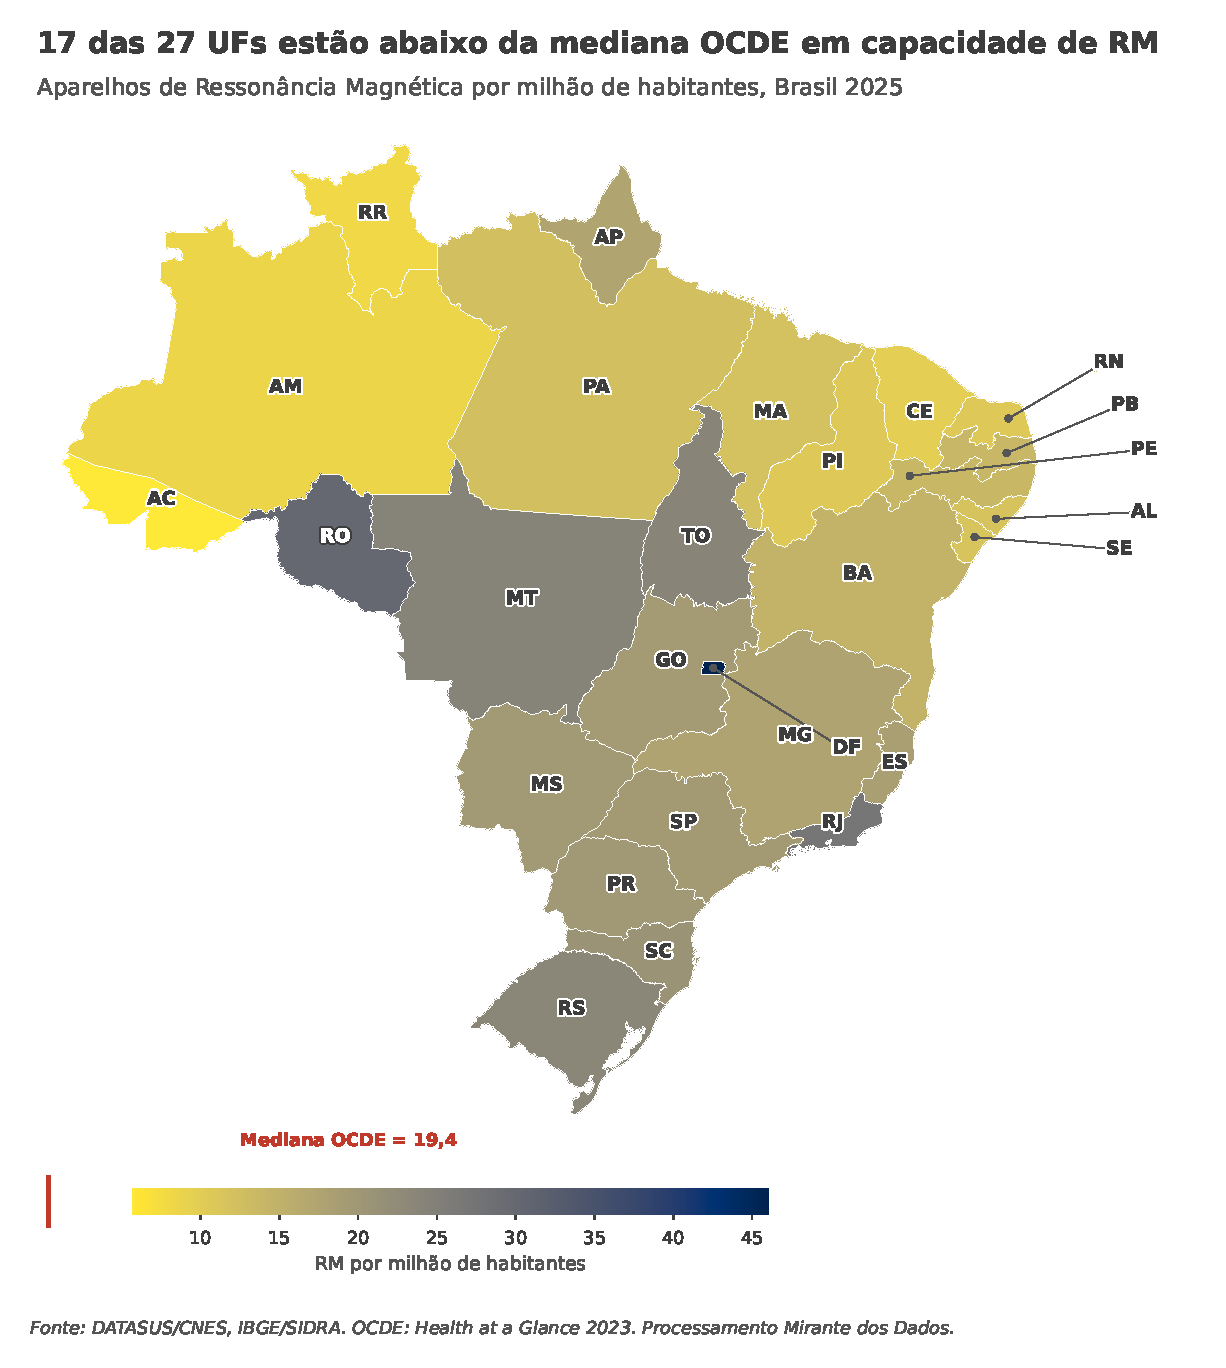
\includegraphics[width=0.72\linewidth]{fig05-choropleth-rm}
\caption{Densidade de ressonância magnética por unidade federativa
(RM/Mhab). Brasil, 2025}
\label{fig:choro}
\par\noindent{\small Fonte: CNES/DATASUS (2025) e IBGE. Tom mais escuro
indica maior densidade.}
\end{figure}

\begin{figure}[htbp]
\centering
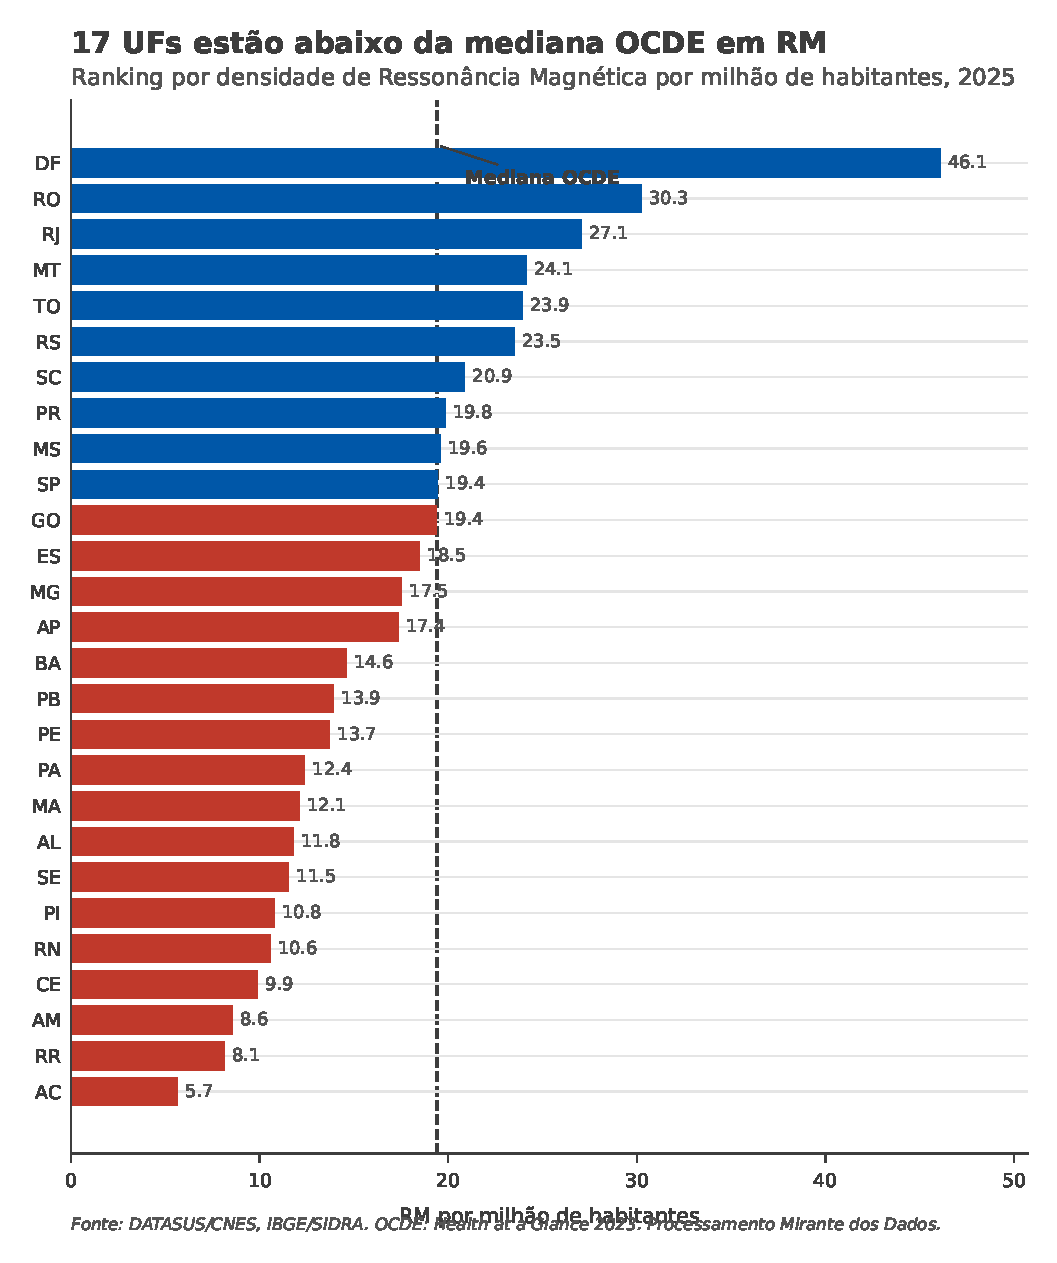
\includegraphics[width=0.76\linewidth]{fig08-top-uf-rm}
\caption{Densidade de ressonância magnética por unidade federativa,
ordenada por valor per capita. Brasil, 2025}
\label{fig:ranking}
\par\noindent{\small Fonte: CNES/DATASUS e IBGE. Linha de referência:
mediana da OCDE ($\approx$19,4/Mhab).}
\end{figure}

A iniquidade, embora persistente, recuou: o coeficiente de variação
inter-UF da densidade de RM caiu de 0,61 (2013) para 0,48 (2025),
redução de 21\%, indicando convergência relativa \textemdash{} a
expansão beneficiou desproporcionalmente UF antes subdotadas. A
convergência, contudo, foi modalidade-dependente: a CT seguiu
trajetória análoga (0,48\,$\rightarrow$\,0,40), enquanto a câmara gama
permaneceu fortemente desigual ao longo de todo o período
(coeficiente de variação $\sim$0,7\textendash 0,8) e a PET/CT, dada a
pequena base instalada e a concentração em capitais, manteve dispersão
elevada \textemdash{} ou seja, a redução da iniquidade restringiu-se às
modalidades de maior difusão e não alcançou a medicina nuclear, da qual
depende a DAT-SPECT. Ainda assim, o índice de Kakwani sobre RM
\textit{versus} IDH foi
$K = +0{,}183$ (IC \textit{bootstrap} 95\%: 0,124\textendash 0,241),
confirmando distribuição regressiva pró-rico; estendido às quatro
modalidades, $K = +0{,}141$ (0,082\textendash 0,198). O índice de
necessidade (Tabela~\ref{tab:necessidade}) mostrou pressão relativa
cerca de oito vezes maior no Acre (584 pacientes estimados de DP por
aparelho) e em Roraima (406) do que no Distrito Federal (72) ou em
Rondônia (109). \textit{A magnitude dessa discrepância indica que a
subdotação de algumas UF não é incremental, mas estrutural.}

\begin{table}[htbp]
\centering
\caption{Índice de necessidade: pacientes estimados de doença de
Parkinson por aparelho de ressonância magnética, unidades federativas
extremas. Brasil, 2025}
\begin{tabular}{lrrr}
\toprule
\textbf{UF} & \textbf{Casos est.\ de DP} & \textbf{RM} & \textbf{DP/RM} \\
\midrule
\multicolumn{4}{l}{\textit{Maior pressão (déficit relativo)}} \\
Acre (AC)                   &  2.918 &   5 & 584 \\
Roraima (RR)                &  2.438 &   6 & 406 \\
Amazonas (AM)               & 14.261 &  37 & 385 \\
Ceará (CE)                  & 30.587 &  92 & 332 \\
Rio Grande do Norte (RN)    & 11.402 &  36 & 317 \\
\midrule
\multicolumn{4}{l}{\textit{Menor pressão (folga relativa)}} \\
Distrito Federal (DF)       &  9.890 & 138 &  72 \\
Rondônia (RO)               &  5.781 &  53 & 109 \\
Rio de Janeiro (RJ)         & 56.838 & 466 & 122 \\
Mato Grosso (MT)            & 12.849 &  94 & 137 \\
Tocantins (TO)              &  5.237 &  38 & 138 \\
\midrule
\textbf{Brasil}       & \textbf{704.290} & \textbf{3.900} & \textbf{181} \\
\bottomrule
\end{tabular}
\par\noindent{\small Fonte: CNES/DATASUS (2025) e IBGE. Casos estimados
$=$ população residente $\times$ 0,33\% (\textit{proxy} conservadora;
ver Métodos).}
\label{tab:necessidade}
\end{table}

% =====================================================================
\section{Discussão}
% =====================================================================

Os resultados qualificam a percepção de que o Brasil estaria
dramaticamente subdotado em RM: na média nacional, o país situa-se
sobre a mediana da OCDE, acima de França, Reino Unido e Canadá. O
problema brasileiro não é o volume agregado, mas a sua
\textbf{distribuição}. E essa distribuição configura
\textbf{iniquidade}, e não mera desigualdade: o índice de Kakwani
positivo demonstra que a oferta acompanha o gradiente socioeconômico
em vez de compensá-lo, e as diferenças Norte\textendash Sudeste não são
atenuadas por mecanismos de equidade \textemdash{} redes robustas de
telerradiologia, fluxos formais de referência ou políticas deliberadas
de interiorização da alta complexidade. Trata-se de uma expressão
local da ``lei dos cuidados inversos'', segundo a qual a oferta de bons
cuidados tende a variar inversamente à necessidade da população
atendida\,[\ref{ref:hart}]; a concentração de RM nas UF de maior IDH,
contraposta à maior pressão de necessidade nas UF do Norte e Nordeste,
materializa essa lei na capacidade diagnóstica para a DP.

A iniquidade aqui documentada não é um fenômeno isolado da
neuroimagem. A distribuição geográfica de equipamentos diagnósticos no
Brasil já é descrita como espacialmente desigual, com vazios
assistenciais persistentes no Norte e em parte do
Nordeste\,[\ref{ref:lopes}], e a literatura de acesso a recursos de
alta complexidade do SUS \textemdash{} leitos de terapia intensiva,
hemodinâmica, radioterapia e medicina nuclear \textemdash{} reporta
padrões análogos de concentração nas unidades federativas de maior
IDH. A iniquidade em neuroimagem para a DP é, assim, manifestação
particular de um padrão sistêmico mais amplo de regionalização
incompleta da alta complexidade, em que a oferta tende a seguir a
capacidade instalada e o mercado privado preexistentes, e não a
necessidade epidemiológica. A consequência para a política pública é
direta: intervenções dirigidas a uma única tecnologia ou a uma única
doença tendem a reproduzir a mesma geografia da iniquidade, ao passo
que correções duradouras dependem de instrumentos transversais de
planejamento regional \textemdash{} definição de regiões de saúde,
parâmetros de cobertura ponderados pela necessidade e fluxos formais
de referência inter-regional \textemdash{} capazes de redistribuir
capacidade diagnóstica de forma deliberada.

Do ponto de vista assistencial, a baixa disponibilidade de RM e de
DAT-SPECT no Norte e em parte do Nordeste compromete a aplicação
prática dos critérios diagnósticos da DP, que pressupõem acesso à
neuroimagem para confirmar ou excluir o diagnóstico em cenários de
incerteza\,[\ref{ref:mds}, \ref{ref:catafau}]. Como a câmara gama
abrange aplicações além da DAT-SPECT, o parque cadastrado é um limite
\textit{superior} da capacidade alocável a esse exame; a fração
efetivamente dedicada à DP é provavelmente menor, o que reforça \textemdash{}
e não enfraquece \textemdash{} o argumento de subcapacidade. A
literatura associa o acesso restrito à neuroimagem ao diagnóstico
tardio, à perda de janela terapêutica e à maior sobrecarga sobre
pacientes e famílias\,[\ref{ref:tolosa}]. Essa cadeia tem
consequências concretas: na ausência de RM e de DAT-SPECT, parte dos
parkinsonismos atípicos é classificada erroneamente como DP idiopática
\textemdash{} ou o inverso \textemdash{}, retardando condutas
específicas, expondo o paciente a ensaios terapêuticos inadequados e
prolongando o intervalo até o diagnóstico correto, com repercussão
sobre incapacidade, qualidade de vida e custos de cuidado assumidos
pelas famílias. Há, ainda, um paradoxo regulatório: os próprios
critérios diagnósticos de referência presumem a disponibilidade de
neuroimagem, de modo que, onde ela falta, o padrão-ouro torna-se
inaplicável e o diagnóstico recai sobre avaliação clínica isolada,
mais sujeita a erro. Assim, a iniquidade aqui documentada no nível das
UF tende a traduzir-se em desigualdades de desfecho para os pacientes
dessas regiões, e não apenas em diferenças de contagem de equipamentos.

Três intervenções poderiam mitigar a iniquidade sem depender da
aquisição de equipamentos de grande porte, articulando-se aos
instrumentos de regulação do SUS e às Redes de Atenção à Saúde. A
\textbf{padronização de um protocolo nacional de RM para DP}
(sequências convencionais, susceptibilidade e difusão) é implementável
no parque já instalado, inclusive em equipamentos de 1,5\,T, alinhada
ao mínimo recomendado pelas diretrizes\,[\ref{ref:efns}]. A
\textbf{capacitação de neurorradiologistas} ampliaria o rendimento
diagnóstico do parque existente\,[\ref{ref:pyatigorskaya}]. E a
\textbf{telerradiologia}, com laudo remoto por centros de excelência
das imagens adquiridas em UF subdotadas, dissociaria a competência
interpretativa da localização do equipamento, em moldes de fluxos
formais de referência e contrarreferência. A capacidade de absorção
dessas medidas é maior que a de uma expansão de PET/CT, cujo custo de
capital e a dependência de cíclotron a restringem a centros
terciários\,[\ref{ref:stoessl}]; a própria RM, equipamento de capital
intensivo que exige resfriamento criogênico contínuo e infraestrutura
dedicada\,[\ref{ref:vogel}], é estruturalmente mais onerosa de instalar
e manter em UF remotas, o que reforça a prioridade de extrair maior
rendimento da capacidade instalada.

Essas medidas encontram amparo nos instrumentos já existentes de
governança do SUS, o que as torna implementáveis sem necessariamente
depender de novos investimentos de capital. O desenho de fluxos de
neuroimagem-DP por macrorregião de saúde, com pactuação de referência e
contrarreferência, é matéria típica do Planejamento Regional Integrado
e da Programação Geral das Ações e Serviços de Saúde; a incorporação de
um protocolo padronizado e do laudo a distância pode ser operacionalizada
pela Política Nacional de Regulação e pelos complexos reguladores
estaduais, e ancorada nas redes temáticas de atenção às condições
crônicas. A leitura distributiva aqui proposta sugere, ainda, que
parâmetros de cobertura ponderados pela necessidade estimada
\textemdash{} e não apenas pela população bruta \textemdash{} seriam
mais aderentes ao princípio da equidade, ao direcionar a expansão para
as UF de maior pressão relativa em vez de acompanhar a capacidade
instalada preexistente.

A urgência é demográfica. O envelhecimento é desigual entre as UF:
regiões hoje com pirâmide etária mais jovem \textemdash{} sobretudo no
Norte \textemdash{} apresentam as maiores taxas projetadas de
crescimento da população idosa nas próximas duas
décadas\,[\ref{ref:ibge-proj}]. A colisão entre esse crescimento e a
infraestrutura hoje mais subdotada ocorrerá justamente onde a oferta é
menor, ampliando a distância entre necessidade e oferta.

Este estudo tem limitações. Por seu \textbf{desenho ecológico}, as
associações observadas referem-se ao nível das UF e não autorizam
inferência causal no nível individual. As contagens do CNES refletem
equipamentos \textit{cadastrados}, não necessariamente em produção
efetiva. O cadastro distingue a quantidade \textit{existente}
(\texttt{QT\_EXIST}, aqui adotada por alinhamento às séries da OCDE) da
quantidade \textit{em uso} (\texttt{QT\_USO}); a diferença
\textemdash{} equipamentos parados ou em manutenção \textemdash{} é
capacidade ociosa que a contagem cadastral não capta, de modo que a
oferta efetivamente operante pode ser menor que a reportada, o que
tenderia a agravar, e não atenuar, a iniquidade. O cruzamento futuro
com bases de produção e com \texttt{QT\_USO} permitiria validar o
cadastro. A impossibilidade de estratificar a RM por intensidade de
campo a partir do CNES limita a leitura clínica fina. A
\textit{proxy} homogênea de carga de DP (0,33\%) subestima a pressão em
UF mais envelhecidas; ajustada pela pirâmide etária de cada UF, a
iniquidade seria provavelmente ainda mais pronunciada nas regiões com
maior proporção de idosos. Por fim, a análise foi conduzida no nível
das UF, embora o CNES registre geografia mais fina (município e Região
de Saúde), o que habilita, em trabalhos futuros, a análise da
iniquidade intra-estadual e o desenho de fluxos regionalizados de
referência.

Em conclusão, entre 2013 e 2025 a densidade média nacional de RM
alcançou a mediana da OCDE, mas essa média esconde uma iniquidade
regional estrutural, regressiva pró-rico e com pressão de necessidade
até oito vezes maior nas regiões mais desassistidas. Os resultados
sustentam fortemente a existência dessa iniquidade espacial; as
intervenções propostas \textemdash{} padronização de protocolo,
capacitação e telerradiologia \textemdash{} são recomendações
plausíveis e de baixo custo relativo, porém não avaliadas
empiricamente neste estudo, e devem ser objeto de pesquisa subsequente.
A barreira ao diagnóstico diferencial da DP no Brasil é, portanto, um
problema rastreável e mensurável de \textit{distribuição} do acesso,
cuja correção exige investimento deliberado e regionalizado em
capacidade diagnóstica, e não apenas crescimento agregado do parque.

% =====================================================================
\section*{Agradecimentos}
% =====================================================================

Ao DATASUS/Ministério da Saúde e ao IBGE, pela disponibilização
pública e gratuita dos dados que tornaram este estudo possível.

% =====================================================================
\section*{Referências}
% =====================================================================
\begin{singlespace}\small

\refitem{ref:gbd}
Steinmetz JD, Seeher KM, Schiess N, et al. Global, regional, and
national burden of disorders affecting the nervous system, 1990--2021:
a systematic analysis for the Global Burden of Disease Study 2021.
Lancet Neurol. 2024;23(4):344-81. DOI: 10.1016/S1474-4422(24)00038-3.
\par\smallskip

\refitem{ref:su}
Su D, Cui Y, He C, et al. Projections for prevalence of Parkinson's
disease and its driving factors in 195 countries and territories to
2050. BMJ. 2025;388:e080952. DOI: 10.1136/bmj-2024-080952.
\par\smallskip

\refitem{ref:marras}
Marras C, Beck JC, Bower JH, et al. Prevalence of Parkinson's disease
across North America. NPJ Parkinsons Dis. 2018;4:21. DOI:
10.1038/s41531-018-0058-0.
\par\smallskip

\refitem{ref:voncamp}
von Campenhausen S, Bornschein B, Wick R, et al. Prevalence and
incidence of Parkinson's disease in Europe. Eur Neuropsychopharmacol.
2005;15(4):473-90. DOI: 10.1016/j.euroneuro.2005.04.007.
\par\smallskip

\refitem{ref:elsi}
Schlickmann TH, Tessari MS, Borelli WV, et al. Prevalence, distribution
and future projections of Parkinson disease in Brazil: insights from
the ELSI-Brazil cohort study. Lancet Reg Health Am. 2025;44:101046.
DOI: 10.1016/j.lana.2025.101046.
\par\smallskip

\refitem{ref:ibge-proj}
Instituto Brasileiro de Geografia e Estatística. Projeções da
população: Brasil e Unidades da Federação --- revisão 2024. Rio de
Janeiro: IBGE; 2024.
\par\smallskip

\refitem{ref:mds}
Postuma RB, Berg D, Stern M, et al. MDS clinical diagnostic criteria
for Parkinson's disease. Mov Disord. 2015;30(12):1591-601. DOI:
10.1002/mds.26424.
\par\smallskip

\refitem{ref:tolosa}
Tolosa E, Garrido A, Scholz SW, Poewe W. Challenges in the diagnosis of
Parkinson's disease. Lancet Neurol. 2021;20(5):385-97. DOI:
10.1016/S1474-4422(21)00030-2.
\par\smallskip

\refitem{ref:efns}
Berardelli A, Wenning GK, Antonini A, et al. EFNS/MDS-ES
recommendations for the diagnosis of Parkinson's disease. Eur J Neurol.
2013;20(1):16-34. DOI: 10.1111/ene.12022.
\par\smallskip

\refitem{ref:aan}
Foti SC, Lashley T, Holton JL, et al. Time for clinical dopamine
transporter scans in parkinsonism? Neurology. 2024;102:e209558. DOI:
10.1212/WNL.0000000000209558.
\par\smallskip

\refitem{ref:swallow}
Mahlknecht P, Krismer F, Poewe W, Seppi K. Meta-analysis of
dorsolateral nigral hyperintensity on MRI as a marker for Parkinson's
disease. Mov Disord. 2017;32(4):619-23. DOI: 10.1002/mds.26932.
\par\smallskip

\refitem{ref:saba}
Saba RA, Maia DP, Cardoso FEC, et al. Guidelines for Parkinson's
disease treatment: consensus from the Movement Disorders Scientific
Department of the Brazilian Academy of Neurology --- motor symptoms.
Arq Neuropsiquiatr. 2022;80(3):316-29. DOI: 10.1590/0004-282X-ANP-2021-0219.
\par\smallskip

\refitem{ref:catafau}
Catafau AM, Tolosa E; DaTSCAN Clinically Uncertain Parkinsonian
Syndromes Study Group. Impact of dopamine transporter SPECT using
123I-Ioflupane on diagnosis and management of patients with clinically
uncertain parkinsonian syndromes. Mov Disord. 2004;19(10):1175-82.
DOI: 10.1002/mds.20112.
\par\smallskip

\refitem{ref:stoessl}
Stoessl AJ, Lehericy S, Strafella AP. Imaging insights into basal
ganglia function, Parkinson's disease, and dystonia. Lancet.
2014;384(9942):532-44. DOI: 10.1016/S0140-6736(14)60041-6.
\par\smallskip

\refitem{ref:lopes}
Lopes VC, Barros MB, Ávila A, et al. Distribuição geográfica de
equipamentos de diagnóstico por imagem no Brasil: análise espacial sob
a ótica do acesso ao SUS. Cad Saúde Pública. 2022;38(3):e00170721.
DOI: 10.1590/0102-311X00170721.
\par\smallskip

\refitem{ref:wagstaff}
Wagstaff A, Paci P, van Doorslaer E. On the measurement of inequalities
in health. Soc Sci Med. 1991;33(5):545-57. DOI: 10.1016/0277-9536(91)90212-U.
\par\smallskip

\refitem{ref:hart}
Hart JT. The inverse care law. Lancet. 1971;297(7696):405-12. DOI:
10.1016/S0140-6736(71)92410-X.
\par\smallskip

\refitem{ref:datasus-cat}
Departamento de Informática do SUS. Catálogo de indicadores de
equipamentos do CNES. Brasília: Ministério da Saúde; [citado 2026 abr
26]. Disponível em:
\url{https://cnes2.datasus.gov.br/Mod_Ind_Equipamento.asp}
\par\smallskip

\refitem{ref:ibge-pop}
Instituto Brasileiro de Geografia e Estatística. Estimativas da
população residente para os municípios e as unidades da federação
(Tabela 6579, SIDRA). Rio de Janeiro: IBGE; 2024.
\par\smallskip

\refitem{ref:lakehouse}
Armbrust M, Ghodsi A, Xin R, Zaharia M. Lakehouse: a new generation of
open platforms that unify data warehousing and advanced analytics. In:
11th Conference on Innovative Data Systems Research (CIDR); 2021.
\par\smallskip

\refitem{ref:oecd}
Organisation for Economic Co-operation and Development. Health at a
Glance 2023: OECD Indicators. Paris: OECD Publishing; 2023.
\par\smallskip

\refitem{ref:oecd-ct}
Organisation for Economic Co-operation and Development. Computed
tomography (CT) scanners (indicator). OECD Health Statistics; 2024.
DOI: 10.1787/data-00541-en.
\par\smallskip

\refitem{ref:cadth}
Canadian Agency for Drugs and Technologies in Health. Canadian Medical
Imaging Inventory 2022--2023. Ottawa: CADTH; 2024.
\par\smallskip

\refitem{ref:japan}
Matsumoto M, Koike S, Kashima S, Awai K. Geographic distribution of CT,
MRI and PET devices in Japan. PLoS One. 2015;10(5):e0126036. DOI:
10.1371/journal.pone.0126036.
\par\smallskip

\refitem{ref:kakwani}
Kakwani NC. Measurement of tax progressivity: an international
comparison. Econ J. 1977;87(345):71-80. DOI: 10.2307/2231833.
\par\smallskip

\refitem{ref:atlas}
Programa das Nações Unidas para o Desenvolvimento; IPEA; Fundação João
Pinheiro. Atlas do Desenvolvimento Humano no Brasil; 2024.
\par\smallskip

\refitem{ref:pyatigorskaya}
Pyatigorskaya N, Magnin B, Mongin M, et al. Comparative study of MRI
biomarkers in the substantia nigra to discriminate idiopathic Parkinson
disease. AJNR Am J Neuroradiol. 2018;39(8):1460-7. DOI: 10.3174/ajnr.A5702.
\par\smallskip

\refitem{ref:vogel}
Vogel JP, Hammitt JK, Stoddart GL, et al. Lifecycle cost analysis of
magnetic resonance imaging systems. Health Aff (Millwood).
2020;39(7):1182-90. DOI: 10.1377/hlthaff.2019.01592.
\par\smallskip

\end{singlespace}

\end{document}
